\chapter{Standaard inhoudtypen} \index{inhoudstypen}
\section{Inhoud aanmaken}
Bij de aanmaak van een nieuwe node moet eerst een inhoudstype worden gekozen.
Hiermee worden de basiskenmerken van de node vastgelegd.

Drupal kent standaard drie verschillende inhoudstypes. De namen van de eerste
twee types worden niet vertaald bij het invoeren van de vertaling van de website.
\begin{itemize}
\item Pagina
\item Verhaal
\item Boek (indien de boekmodule ingeschakeld is).
\end{itemize}

\subsection{pagina} \index{pagina} \index{page}
Bedoeld voor een statische pagina \footnote{In de vertaalde website staat
'page'}, zoals een contactpagina of een 'over ons' pagina.

\subsection{verhaal} \index{verhaal} \index{story}
Verhalen \footnote{In de vertaalde website staat 'story'} zijn de meest simpele
artikelen: ze hebben een titel, een voorproefje en een berichttekst. Andere modules 
kunnen meer eigenschappen toevoegen. Het voorproefje is een integraal onderdeel van de 
berichttekst. Verhalen kunnen gebruikt worden voor een persoonlijke blog, voor nieuwsartikelen of een kort bericht.
De standaardinstelling is dat een verhaal op de voorpagina wordt gepubliceerd.

\subsection{Boek} \index{boek}

Een boek \footnote{In de vertaalde website staat 'book page'} is een
gezamenlijke schrijfinspanning: gebruikers kunnen samen de pagina's van het boek
schrijven, de pagina's in de juiste volgorde plaatsen en eerder geschreven
pagina's nalezen en verbeteren. Wanneer u informatie wilt delen, of een pagina van een boek leest die u niet bevalt, of denkt dat u een 
bepaalde pagina beter kunt schrijven, kunt u er zelf iets aan doen.
\\
Boekpagina's zijn automatisch voorzien van links naar aangrenzende pagina's en hebben daarmee een eenvoudig navigatiesysteem.


\section{Inhoudtypen}
Als voorbeeld gebruik ik het 'boekpagina' type.
 \begin{figure}[!h]
    \centering
   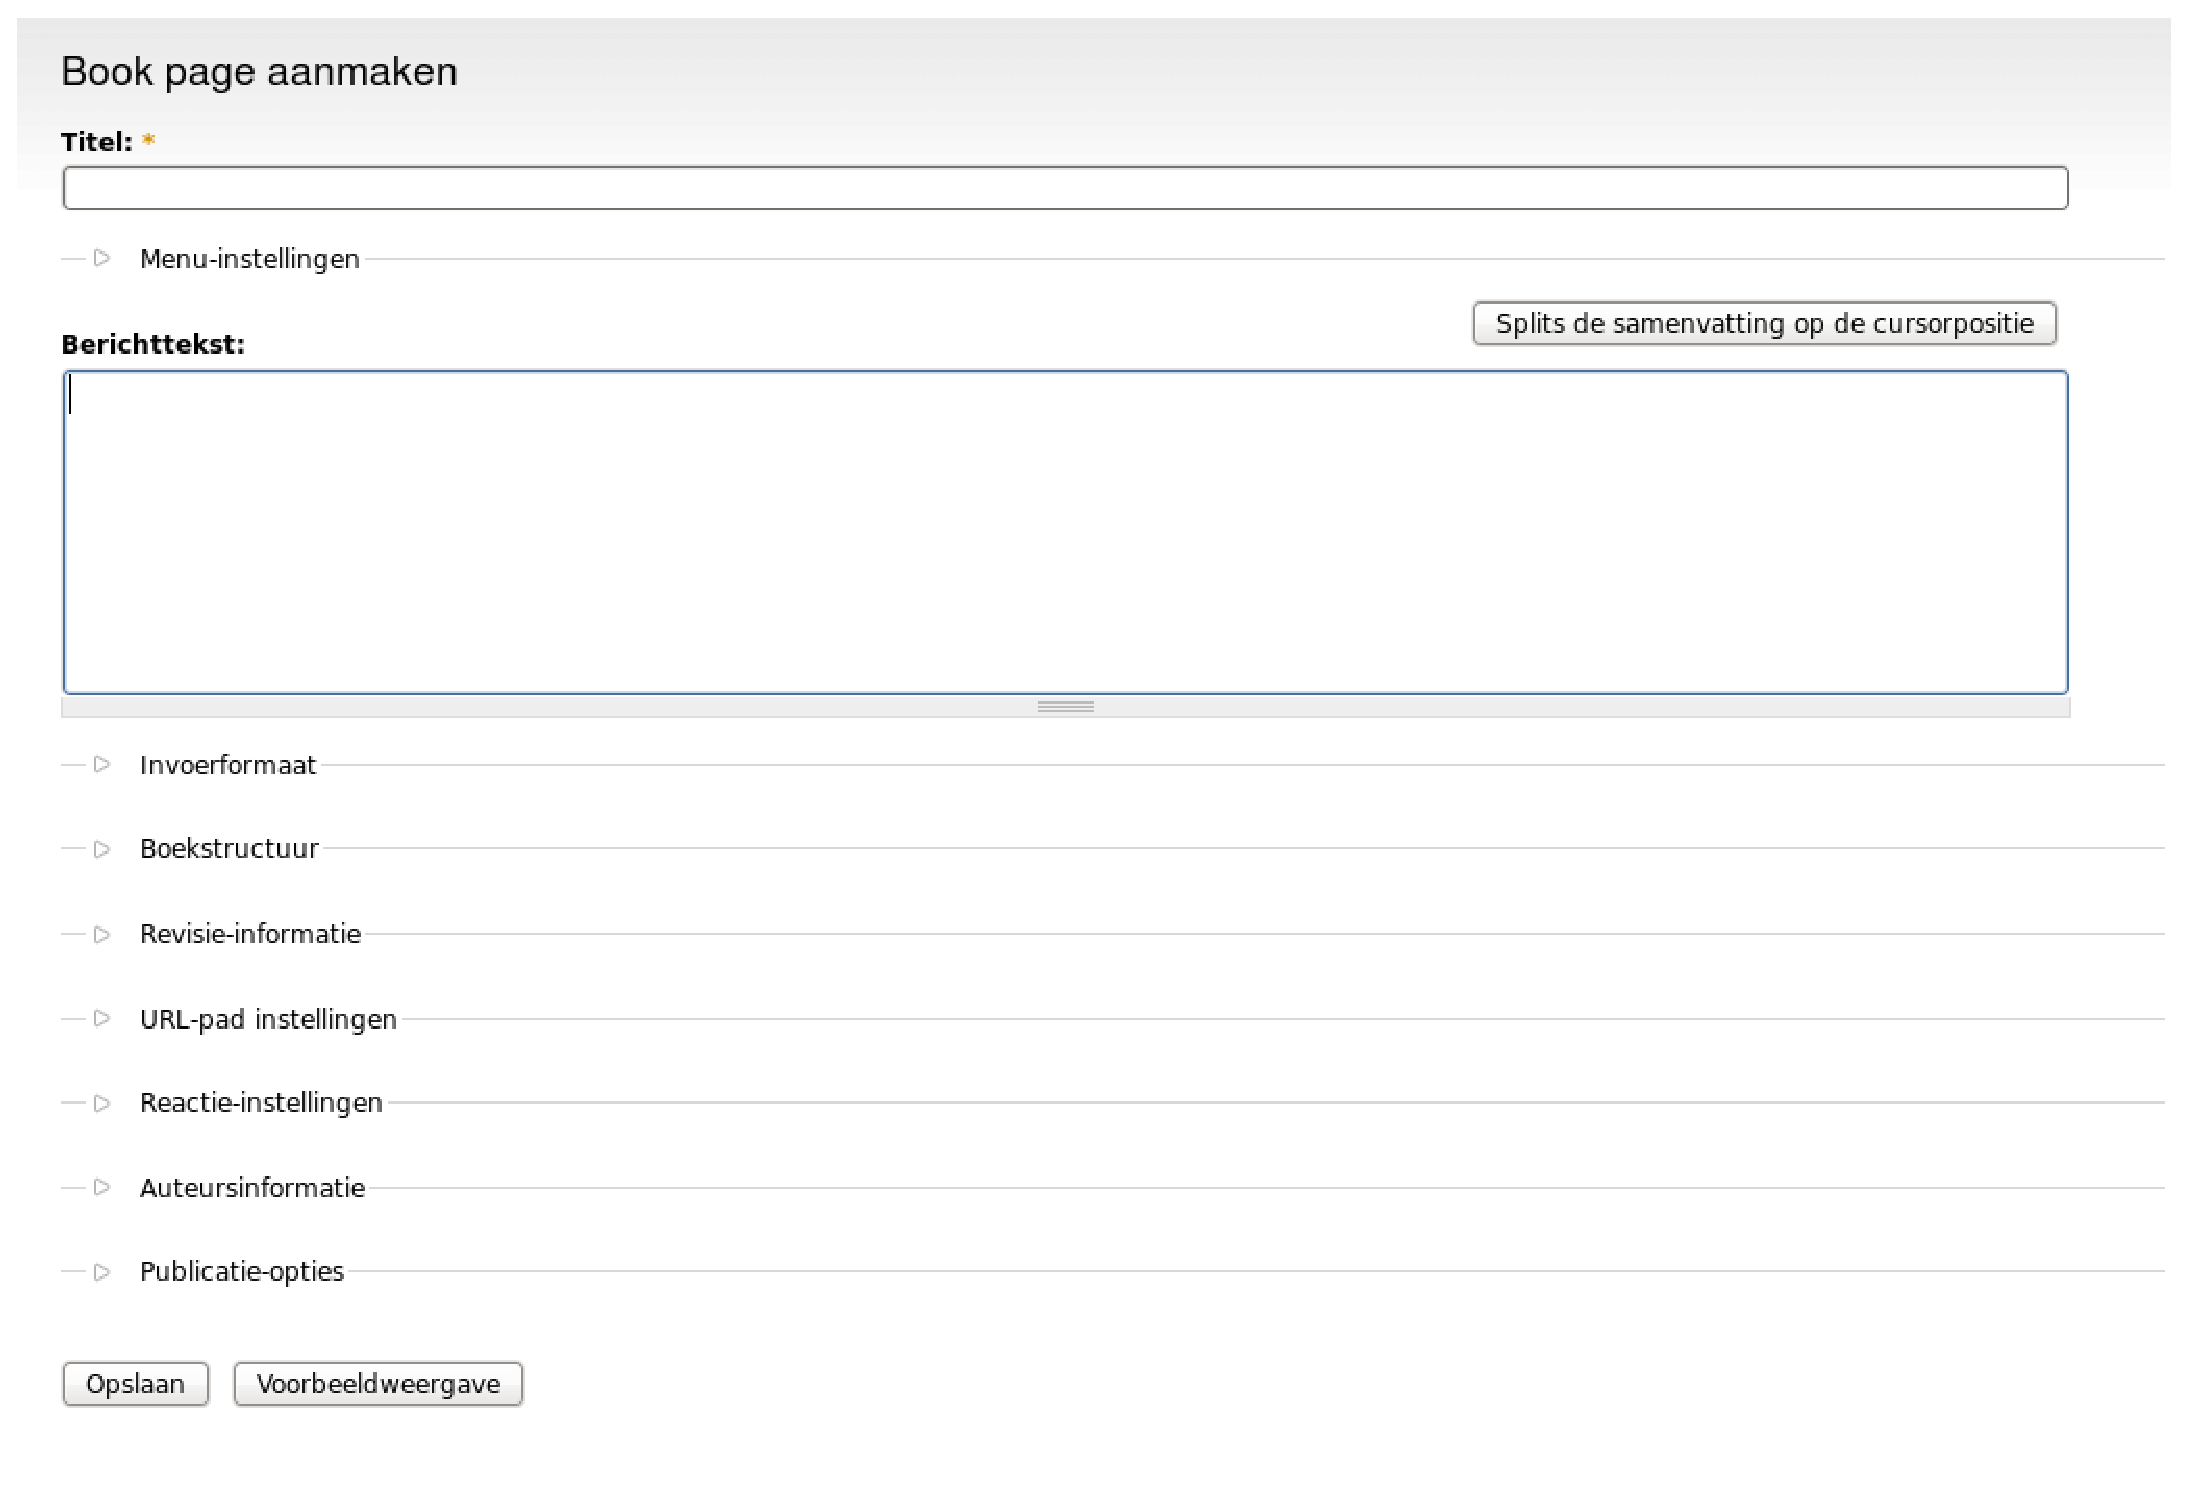
\includegraphics[scale=0.3,angle=0]{book_page_aanmaken}
   \caption{Boek pagina aanmaken.\label{white}}
 \end{figure}

\subsection{Menu-instellingen} \index{menu-instellingen}
De kenmerken van ieder inhoudstype is simpel aan te passen.
 \begin{figure}[!h]
    \centering
   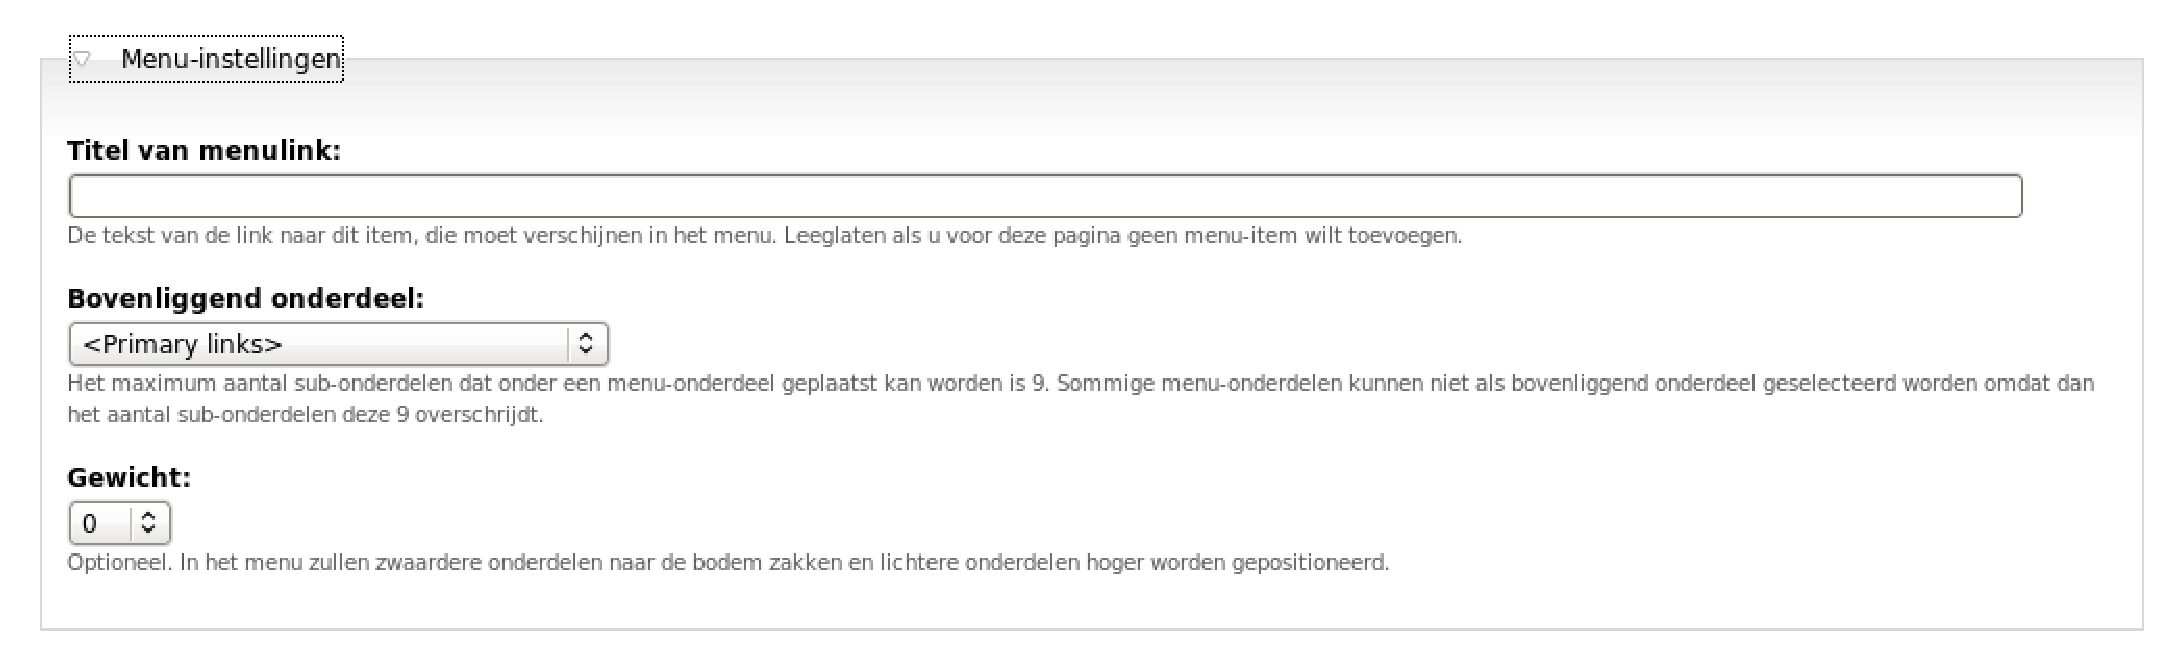
\includegraphics[scale=0.3,angle=0]{menu-instellingen}
   \caption{Menu-instellingen.\label{white}}
 \end{figure}
\begin{itemize}
  \item  Titel van menulink: \index{menulink} De tekst van de link
  \index{link} naar dit item, die moet verschijnen in het menu. Leeglaten als u
  voor deze pagina geen menu-item wilt toevoegen.
  \item  Bovenliggend onderdeel: Het maximum aantal sub-onderdelen dat onder een
  menu-onderdeel geplaatst kan worden is 9. Sommige menu-onderdelen kunnen niet als bovenliggend 
  onderdeel geselecteerd worden omdat dan het aantal sub-onderdelen deze 9 overschrijdt.
  \begin{figure}[!h]
    \centering
   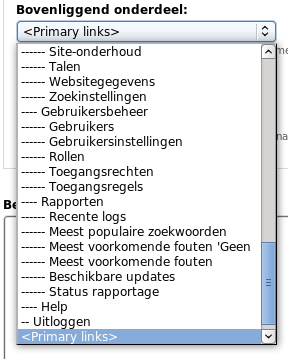
\includegraphics[scale=0.3,angle=0]{bovenliggend-onderdeel}
   \caption{bovenliggend-onderdeel.\label{white}}
 \end{figure}
  \item  Gewicht: Optioneel. In het menu zullen zwaardere onderdelen naar de
  bodem zakken en lichtere onderdelen hoger worden gepositioneerd.
\end{itemize}

\subsection{Invoerformaat} \index{invoerformaat}

 \begin{figure}[!h]
    \centering
   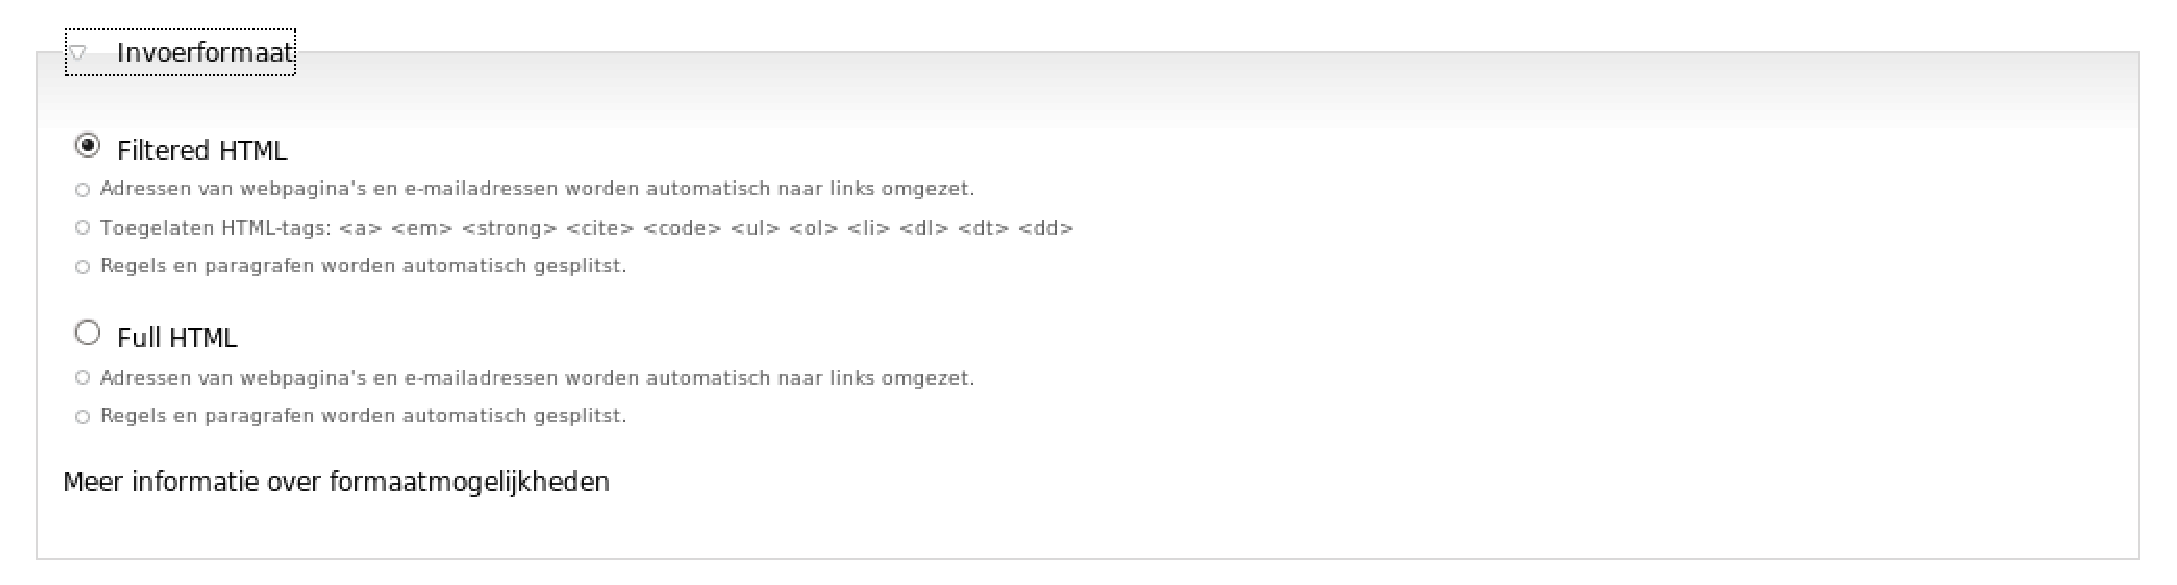
\includegraphics[scale=0.3,angle=0]{invoerformaat}
   \caption{Invoerformaat.\label{white}}
 \end{figure}
Filtered HTML \index{filtered html} \index{html}
        \begin{itemize}
            \item Adressen van webpagina's en e-mailadressen worden automatisch naar links omgezet.
            \item Toegelaten HTML-tags: $<$a$>$ $<$em$>$ $<$strong$>$ $<$cite$>$
            $<$code$>$ $<$ul$>$ $<$ol$>$ $<$li$>$ $<$dl$>$ $<$dt$>$ $<$dd$>$
            \item Regels en paragrafen worden automatisch gesplitst.
        \end{itemize} 
Full HTML \index{full-html}
        \begin{itemize}
            \item Adressen van webpagina's en e-mailadressen worden automatisch
            naar links omgezet.
            \item Regels en paragrafen worden automatisch gesplitst.
        \end{itemize}

\subsection{Boekstructuur} \index{boekstructuur}
 \begin{figure}[!h]
    \centering
   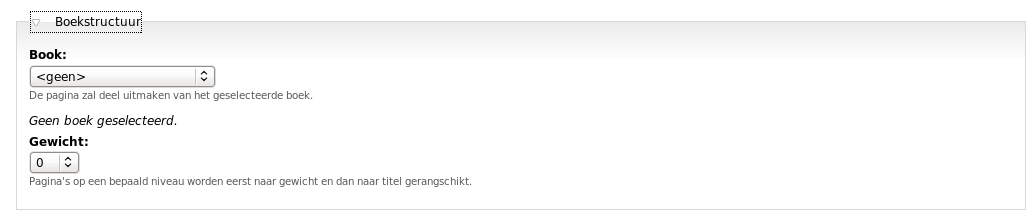
\includegraphics[scale=0.3,angle=0]{boekstructuur}
   \caption{Boekstructuur.\label{white}}
 \end{figure}
\begin{itemize}
  \item Book: De pagina zal deel uitmaken van het geselecteerde boek.
  \item Gewicht: \index{gewicht} Pagina's op een bepaald niveau worden eerst
  naar gewicht en dan naar titel gerangschikt.
\end{itemize}

\subsection{Revisie-informatie} \index{revisie-informatie}
 \begin{figure}[!h]
    \centering
   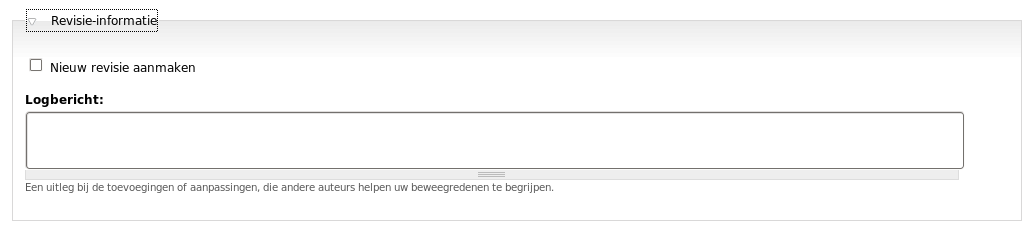
\includegraphics[scale=0.3,angle=0]{revisie-informatie}
   \caption{Revisie-informatie.\label{white}}
 \end{figure}
Hier kan je een nieuw revisie aanmaken. In het logbericht geef je uitleg
bij de toevoegingen of aanpassingen, die andere auteurs helpen uw beweegredenen te begrijpen.

\subsection{URL-pad-instellingen} \index{url-pad}
 \begin{figure}[!h]
    \centering
   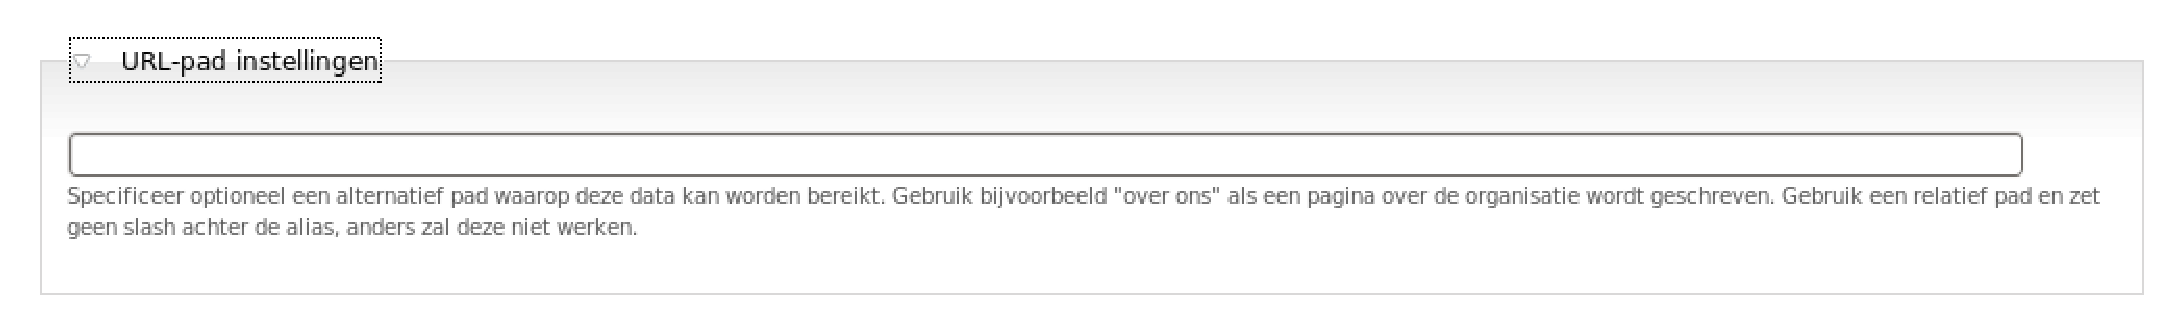
\includegraphics[scale=0.3,angle=0]{url-pad-instellingen}
   \caption{URL-pad-instellingen.\label{white}}
 \end{figure}
Specificeer optioneel een alternatief pad waarop deze data kan worden bereikt.
Gebruik bijvoorbeeld ''over ons'' als een pagina over de organisatie wordt
geschreven. Gebruik een relatief pad en zet geen slash achter de alias, anders zal deze niet werken.

\subsection{Reactie-instellingen} \index{reactie-instellingen}
Hier dient U een titel op te geven, dit is een verplicht veld.
 \begin{figure}[!h]
    \centering
   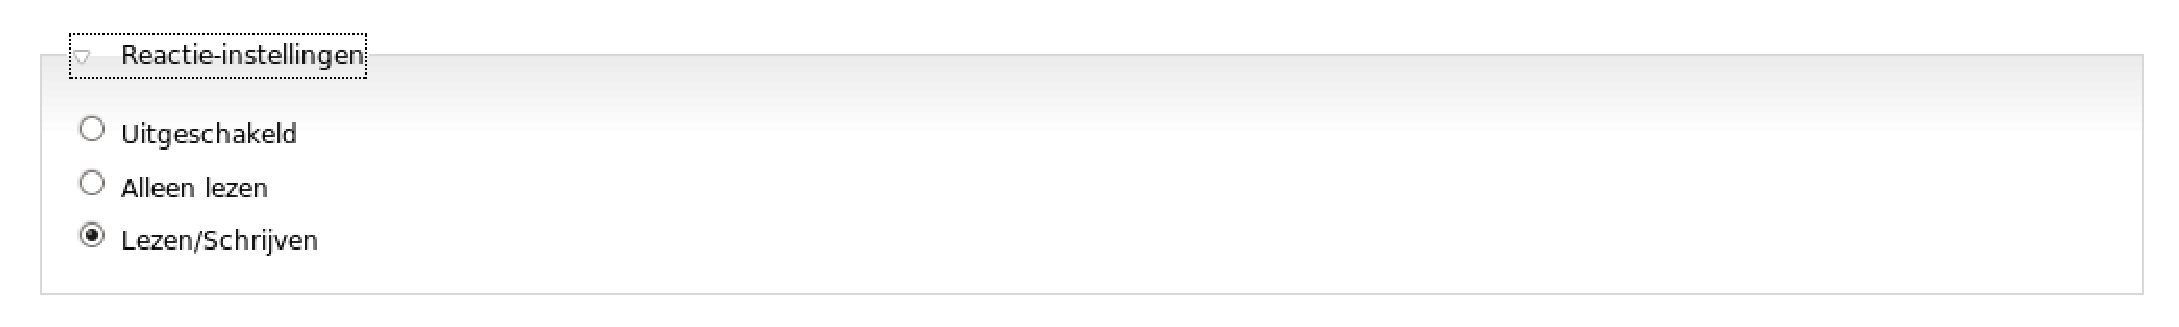
\includegraphics[scale=0.3,angle=0]{reactie-instellingen}
   \caption{Reactie-instellingen.\label{white}}
 \end{figure}
\begin{itemize}
  \item Uitgeschakeld
  \item Alleen lezen
  \item Lezen/Schrijven
\end{itemize}

\subsection{Auteursinformatie} \index{auteursinformatie}
Hier dient U een titel op te geven, dit is een verplicht veld.
 \begin{figure}[!h]
    \centering
   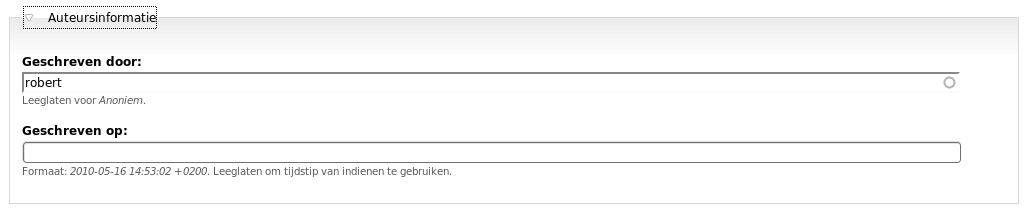
\includegraphics[scale=0.3,angle=0]{auteursinformatie}
   \caption{Auteursinformatie.\label{white}}
 \end{figure}
Hier schrijf je de naam van de auteur en tijdstip van indienen.

\subsection{Publicatie-opties} \index{publicatie-opties}
Hier dient U een titel op te geven, dit is een verplicht veld.
 \begin{figure}[!h]
    \centering
   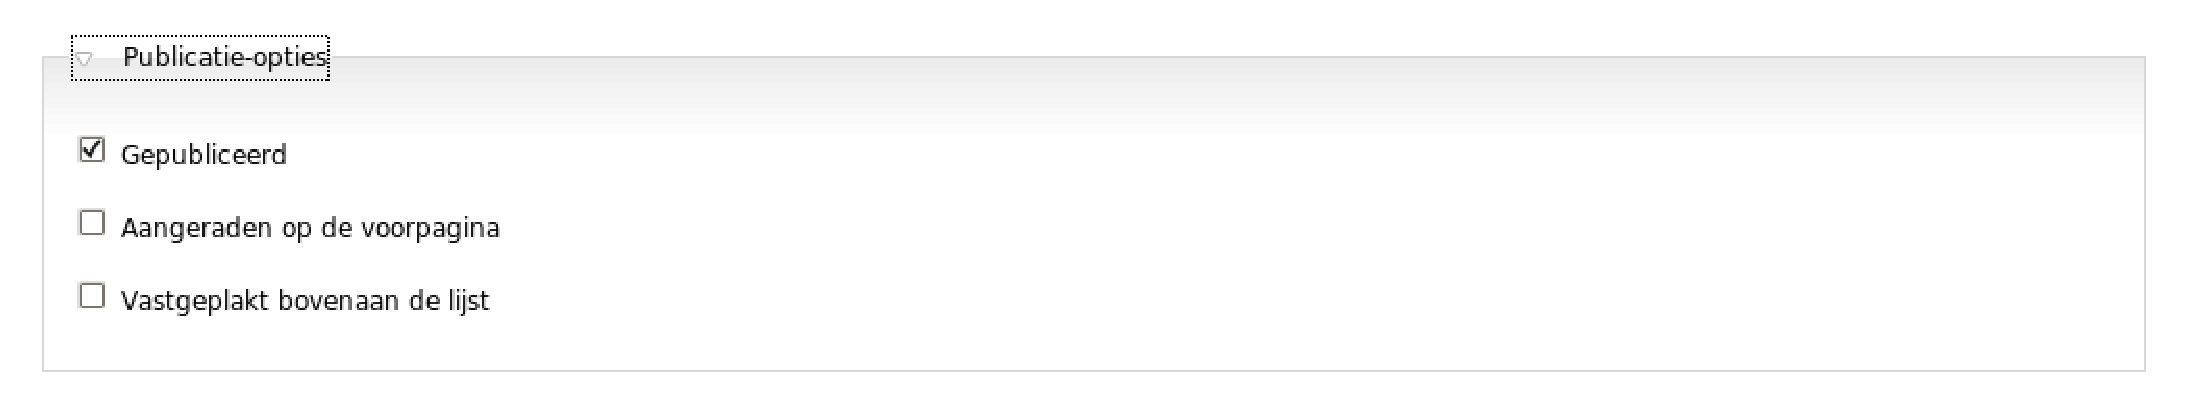
\includegraphics[scale=0.3,angle=0]{publicatie-opties}
   \caption{Publicatie-opties.\label{white}}
 \end{figure}
\begin{itemize}
  \item Gepubliceerd
  \item Aangeraden op de voorpagina
  \item Vastgeplakt bovenaan de lijst
\end{itemize}


